\documentclass[twoside]{book}

% Packages required by doxygen
\usepackage{fixltx2e}
\usepackage{calc}
\usepackage{doxygen}
\usepackage[export]{adjustbox} % also loads graphicx
\usepackage{graphicx}
\usepackage[utf8]{inputenc}
\usepackage{makeidx}
\usepackage{multicol}
\usepackage{multirow}
\PassOptionsToPackage{warn}{textcomp}
\usepackage{textcomp}
\usepackage[nointegrals]{wasysym}
\usepackage[table]{xcolor}

% Font selection
\usepackage[T1]{fontenc}
\usepackage[scaled=.90]{helvet}
\usepackage{courier}
\usepackage{amssymb}
\usepackage{sectsty}
\renewcommand{\familydefault}{\sfdefault}
\allsectionsfont{%
  \fontseries{bc}\selectfont%
  \color{darkgray}%
}
\renewcommand{\DoxyLabelFont}{%
  \fontseries{bc}\selectfont%
  \color{darkgray}%
}
\newcommand{\+}{\discretionary{\mbox{\scriptsize$\hookleftarrow$}}{}{}}

% Page & text layout
\usepackage{geometry}
\geometry{%
  a4paper,%
  top=2.5cm,%
  bottom=2.5cm,%
  left=2.5cm,%
  right=2.5cm%
}
\tolerance=750
\hfuzz=15pt
\hbadness=750
\setlength{\emergencystretch}{15pt}
\setlength{\parindent}{0cm}
\setlength{\parskip}{3ex plus 2ex minus 2ex}
\makeatletter
\renewcommand{\paragraph}{%
  \@startsection{paragraph}{4}{0ex}{-1.0ex}{1.0ex}{%
    \normalfont\normalsize\bfseries\SS@parafont%
  }%
}
\renewcommand{\subparagraph}{%
  \@startsection{subparagraph}{5}{0ex}{-1.0ex}{1.0ex}{%
    \normalfont\normalsize\bfseries\SS@subparafont%
  }%
}
\makeatother

% Headers & footers
\usepackage{fancyhdr}
\pagestyle{fancyplain}
\fancyhead[LE]{\fancyplain{}{\bfseries\thepage}}
\fancyhead[CE]{\fancyplain{}{}}
\fancyhead[RE]{\fancyplain{}{\bfseries\leftmark}}
\fancyhead[LO]{\fancyplain{}{\bfseries\rightmark}}
\fancyhead[CO]{\fancyplain{}{}}
\fancyhead[RO]{\fancyplain{}{\bfseries\thepage}}
\fancyfoot[LE]{\fancyplain{}{}}
\fancyfoot[CE]{\fancyplain{}{}}
\fancyfoot[RE]{\fancyplain{}{\bfseries\scriptsize Generated by Doxygen }}
\fancyfoot[LO]{\fancyplain{}{\bfseries\scriptsize Generated by Doxygen }}
\fancyfoot[CO]{\fancyplain{}{}}
\fancyfoot[RO]{\fancyplain{}{}}
\renewcommand{\footrulewidth}{0.4pt}
\renewcommand{\chaptermark}[1]{%
  \markboth{#1}{}%
}
\renewcommand{\sectionmark}[1]{%
  \markright{\thesection\ #1}%
}

% Indices & bibliography
\usepackage{natbib}
\usepackage[titles]{tocloft}
\setcounter{tocdepth}{3}
\setcounter{secnumdepth}{5}
\makeindex

% Hyperlinks (required, but should be loaded last)
\usepackage{ifpdf}
\ifpdf
  \usepackage[pdftex,pagebackref=true]{hyperref}
\else
  \usepackage[ps2pdf,pagebackref=true]{hyperref}
\fi
\hypersetup{%
  colorlinks=true,%
  linkcolor=blue,%
  citecolor=blue,%
  unicode%
}

% Custom commands
\newcommand{\clearemptydoublepage}{%
  \newpage{\pagestyle{empty}\cleardoublepage}%
}

\usepackage{caption}
\captionsetup{labelsep=space,justification=centering,font={bf},singlelinecheck=off,skip=4pt,position=top}

%===== C O N T E N T S =====

\begin{document}

% Titlepage & ToC
\hypersetup{pageanchor=false,
             bookmarksnumbered=true,
             pdfencoding=unicode
            }
\pagenumbering{alph}
\begin{titlepage}
\vspace*{7cm}
\begin{center}%
{\Large My Project \\[1ex]\large 1 }\\
\vspace*{1cm}
{\large Generated by Doxygen 1.8.13}\\
\end{center}
\end{titlepage}
\clearemptydoublepage
\pagenumbering{roman}
\tableofcontents
\clearemptydoublepage
\pagenumbering{arabic}
\hypersetup{pageanchor=true}

%--- Begin generated contents ---
\chapter{Class Index}
\section{Class List}
Here are the classes, structs, unions and interfaces with brief descriptions\+:\begin{DoxyCompactList}
\item\contentsline{section}{\hyperlink{class_a_v_l_tree}{A\+V\+L\+Tree} \\*Class for A\+VL Tree }{\pageref{class_a_v_l_tree}}{}
\item\contentsline{section}{\hyperlink{structnode}{node} }{\pageref{structnode}}{}
\item\contentsline{section}{\hyperlink{class_node}{Node} }{\pageref{class_node}}{}
\item\contentsline{section}{\hyperlink{struct_r_b_t_node}{R\+B\+T\+Node} \\*\hyperlink{struct_r_b_t_node}{R\+B\+T\+Node} for red black tree }{\pageref{struct_r_b_t_node}}{}
\item\contentsline{section}{\hyperlink{class_r_b_tree}{R\+B\+Tree} \\*Class to represent Red-\/\+Black Tree }{\pageref{class_r_b_tree}}{}
\end{DoxyCompactList}

\chapter{File Index}
\section{File List}
Here is a list of all files with brief descriptions\+:\begin{DoxyCompactList}
\item\contentsline{section}{/home/kavya/\+Desktop/csn261\+\_\+lab\+\_\+assignment1/q1/code/\hyperlink{q1_8c}{q1.\+c} }{\pageref{q1_8c}}{}
\end{DoxyCompactList}

\chapter{Class Documentation}
\hypertarget{struct_node}{}\section{Node Struct Reference}
\label{struct_node}\index{Node@{Node}}
\subsection*{Public Attributes}
\begin{DoxyCompactItemize}
\item 
int \hyperlink{struct_node_a2fdf3febffa37539c09d0a282525033a}{a}
\item 
int \hyperlink{struct_node_a26cb9e26541900f36489bf503338ce4e}{b} \mbox{[}100\mbox{]}
\item 
int \hyperlink{struct_node_acc103d220defd2fdb5aac8e3b03424c6}{size} = 0
\end{DoxyCompactItemize}


\subsection{Detailed Description}


Definition at line 7 of file q1.\+cpp.



\subsection{Member Data Documentation}
\mbox{\Hypertarget{struct_node_a2fdf3febffa37539c09d0a282525033a}\label{struct_node_a2fdf3febffa37539c09d0a282525033a}} 
\index{Node@{Node}!a@{a}}
\index{a@{a}!Node@{Node}}
\subsubsection{\texorpdfstring{a}{a}}
{\footnotesize\ttfamily int Node\+::a}



Definition at line 9 of file q1.\+cpp.

\mbox{\Hypertarget{struct_node_a26cb9e26541900f36489bf503338ce4e}\label{struct_node_a26cb9e26541900f36489bf503338ce4e}} 
\index{Node@{Node}!b@{b}}
\index{b@{b}!Node@{Node}}
\subsubsection{\texorpdfstring{b}{b}}
{\footnotesize\ttfamily int Node\+::b\mbox{[}100\mbox{]}}



Definition at line 10 of file q1.\+cpp.

\mbox{\Hypertarget{struct_node_acc103d220defd2fdb5aac8e3b03424c6}\label{struct_node_acc103d220defd2fdb5aac8e3b03424c6}} 
\index{Node@{Node}!size@{size}}
\index{size@{size}!Node@{Node}}
\subsubsection{\texorpdfstring{size}{size}}
{\footnotesize\ttfamily int Node\+::size = 0}



Definition at line 11 of file q1.\+cpp.



The documentation for this struct was generated from the following file\+:\begin{DoxyCompactItemize}
\item 
code/\hyperlink{q1_8cpp}{q1.\+cpp}\end{DoxyCompactItemize}

\chapter{File Documentation}
\hypertarget{q2_8cpp}{}\section{code/q2.cpp File Reference}
\label{q2_8cpp}\index{code/q2.\+cpp@{code/q2.\+cpp}}
{\ttfamily \#include $<$bits/stdc++.\+h$>$}\newline
{\ttfamily \#include $<$iostream$>$}\newline
{\ttfamily \#include $<$string$>$}\newline
{\ttfamily \#include $<$fstream$>$}\newline
{\ttfamily \#include $<$sstream$>$}\newline
{\ttfamily \#include $<$vector$>$}\newline
Include dependency graph for q2.\+cpp\+:
\nopagebreak
\begin{figure}[H]
\begin{center}
\leavevmode
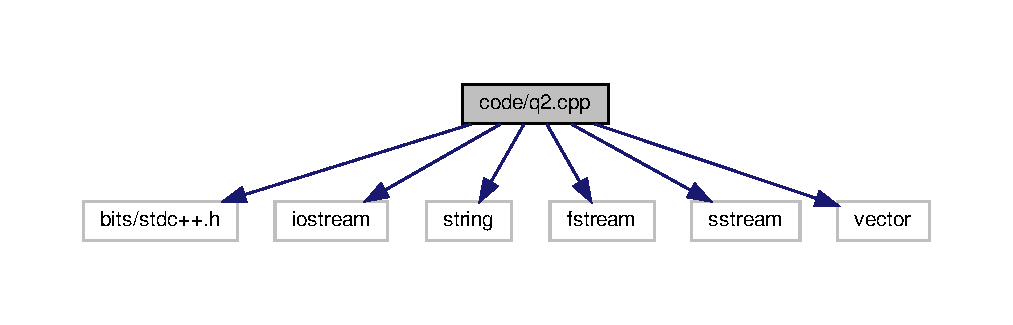
\includegraphics[width=350pt]{q2_8cpp__incl}
\end{center}
\end{figure}
\subsection*{Classes}
\begin{DoxyCompactItemize}
\item 
struct \hyperlink{struct_node}{Node}
\end{DoxyCompactItemize}
\subsection*{Functions}
\begin{DoxyCompactItemize}
\item 
\hyperlink{struct_node}{Node} $\ast$ \hyperlink{q2_8cpp_a0a4979e2df84bd231a92a561ac4d9786}{newnode} (int dat)
\item 
\hyperlink{struct_node}{Node} $\ast$ \hyperlink{q2_8cpp_aea3ba815ab379af020c7e950fe9c3bcc}{merg} (\hyperlink{struct_node}{Node} $\ast$head, \hyperlink{struct_node}{Node} $\ast$p)
\item 
\hyperlink{struct_node}{Node} $\ast$ \hyperlink{q2_8cpp_a64193d0317e37d277f0c01d74f023198}{makeheap} (\hyperlink{struct_node}{Node} $\ast$$\ast$head, \hyperlink{struct_node}{Node} $\ast$$\ast$temp)
\item 
\hyperlink{struct_node}{Node} $\ast$ \hyperlink{q2_8cpp_ac2e791d4fa6bfb659712cff02f42c3e8}{iniheap} (int a\mbox{[}$\,$\mbox{]}, int n, \hyperlink{struct_node}{Node} $\ast$head)
\item 
void \hyperlink{q2_8cpp_a97920b63557b9f137c7e3fa24d7c2a63}{Print} (\hyperlink{struct_node}{Node} $\ast$m, int j)
\item 
void \hyperlink{q2_8cpp_a958dc9f77226b54e52dedf4b23b40760}{M} (ofstream \&fout, \hyperlink{struct_node}{Node} $\ast$head, \hyperlink{struct_node}{Node} $\ast$q)
\item 
int \hyperlink{q2_8cpp_ae66f6b31b5ad750f1fe042a706a4e3d4}{main} ()
\end{DoxyCompactItemize}


\subsection{Function Documentation}
\mbox{\Hypertarget{q2_8cpp_ac2e791d4fa6bfb659712cff02f42c3e8}\label{q2_8cpp_ac2e791d4fa6bfb659712cff02f42c3e8}} 
\index{q2.\+cpp@{q2.\+cpp}!iniheap@{iniheap}}
\index{iniheap@{iniheap}!q2.\+cpp@{q2.\+cpp}}
\subsubsection{\texorpdfstring{iniheap()}{iniheap()}}
{\footnotesize\ttfamily \hyperlink{struct_node}{Node}$\ast$ iniheap (\begin{DoxyParamCaption}\item[{int}]{a\mbox{[}$\,$\mbox{]},  }\item[{int}]{n,  }\item[{\hyperlink{struct_node}{Node} $\ast$}]{head }\end{DoxyParamCaption})}



Definition at line 120 of file q2.\+cpp.

\mbox{\Hypertarget{q2_8cpp_a958dc9f77226b54e52dedf4b23b40760}\label{q2_8cpp_a958dc9f77226b54e52dedf4b23b40760}} 
\index{q2.\+cpp@{q2.\+cpp}!M@{M}}
\index{M@{M}!q2.\+cpp@{q2.\+cpp}}
\subsubsection{\texorpdfstring{M()}{M()}}
{\footnotesize\ttfamily void M (\begin{DoxyParamCaption}\item[{ofstream \&}]{fout,  }\item[{\hyperlink{struct_node}{Node} $\ast$}]{head,  }\item[{\hyperlink{struct_node}{Node} $\ast$}]{q }\end{DoxyParamCaption})}



Definition at line 153 of file q2.\+cpp.

\mbox{\Hypertarget{q2_8cpp_ae66f6b31b5ad750f1fe042a706a4e3d4}\label{q2_8cpp_ae66f6b31b5ad750f1fe042a706a4e3d4}} 
\index{q2.\+cpp@{q2.\+cpp}!main@{main}}
\index{main@{main}!q2.\+cpp@{q2.\+cpp}}
\subsubsection{\texorpdfstring{main()}{main()}}
{\footnotesize\ttfamily int main (\begin{DoxyParamCaption}{ }\end{DoxyParamCaption})}



Definition at line 184 of file q2.\+cpp.

\mbox{\Hypertarget{q2_8cpp_a64193d0317e37d277f0c01d74f023198}\label{q2_8cpp_a64193d0317e37d277f0c01d74f023198}} 
\index{q2.\+cpp@{q2.\+cpp}!makeheap@{makeheap}}
\index{makeheap@{makeheap}!q2.\+cpp@{q2.\+cpp}}
\subsubsection{\texorpdfstring{makeheap()}{makeheap()}}
{\footnotesize\ttfamily \hyperlink{struct_node}{Node}$\ast$ makeheap (\begin{DoxyParamCaption}\item[{\hyperlink{struct_node}{Node} $\ast$$\ast$}]{head,  }\item[{\hyperlink{struct_node}{Node} $\ast$$\ast$}]{temp }\end{DoxyParamCaption})}



Definition at line 98 of file q2.\+cpp.

\mbox{\Hypertarget{q2_8cpp_aea3ba815ab379af020c7e950fe9c3bcc}\label{q2_8cpp_aea3ba815ab379af020c7e950fe9c3bcc}} 
\index{q2.\+cpp@{q2.\+cpp}!merg@{merg}}
\index{merg@{merg}!q2.\+cpp@{q2.\+cpp}}
\subsubsection{\texorpdfstring{merg()}{merg()}}
{\footnotesize\ttfamily \hyperlink{struct_node}{Node}$\ast$ merg (\begin{DoxyParamCaption}\item[{\hyperlink{struct_node}{Node} $\ast$}]{head,  }\item[{\hyperlink{struct_node}{Node} $\ast$}]{p }\end{DoxyParamCaption})}



Definition at line 25 of file q2.\+cpp.

\mbox{\Hypertarget{q2_8cpp_a0a4979e2df84bd231a92a561ac4d9786}\label{q2_8cpp_a0a4979e2df84bd231a92a561ac4d9786}} 
\index{q2.\+cpp@{q2.\+cpp}!newnode@{newnode}}
\index{newnode@{newnode}!q2.\+cpp@{q2.\+cpp}}
\subsubsection{\texorpdfstring{newnode()}{newnode()}}
{\footnotesize\ttfamily \hyperlink{struct_node}{Node}$\ast$ newnode (\begin{DoxyParamCaption}\item[{int}]{dat }\end{DoxyParamCaption})}



Definition at line 16 of file q2.\+cpp.

\mbox{\Hypertarget{q2_8cpp_a97920b63557b9f137c7e3fa24d7c2a63}\label{q2_8cpp_a97920b63557b9f137c7e3fa24d7c2a63}} 
\index{q2.\+cpp@{q2.\+cpp}!Print@{Print}}
\index{Print@{Print}!q2.\+cpp@{q2.\+cpp}}
\subsubsection{\texorpdfstring{Print()}{Print()}}
{\footnotesize\ttfamily void Print (\begin{DoxyParamCaption}\item[{\hyperlink{struct_node}{Node} $\ast$}]{m,  }\item[{int}]{j }\end{DoxyParamCaption})}



Definition at line 134 of file q2.\+cpp.


%--- End generated contents ---

% Index
\backmatter
\newpage
\phantomsection
\clearemptydoublepage
\addcontentsline{toc}{chapter}{Index}
\printindex

\end{document}
